%! suppress = TooLargeSection
\documentclass[conference]{IEEEtran}
\usepackage{cite}
%\usepackage{amsmath,amssymb,amsfonts}
\usepackage{algorithmic}
\usepackage{graphicx}
\usepackage{textcomp}
\usepackage{xcolor}

\usepackage{subfig}
\usepackage[hidelinks]{hyperref}
\graphicspath{ {images/} }
\usepackage{pgfplots}
\pgfplotsset{compat=1.17}

\newcommand\BibTeX{{\textrm{B} \kern-.05em{\textsc{i} \kern-.025em b}\kern-.08em
T\kern-.1667em\lower.7ex\hbox{E}\ker,n-.125emX}}

\begin{document}

    \title{Clothing Item Generation using GANs}

    \author{\IEEEauthorblockN{Charlie Brayton (014559415)}
    \IEEEauthorblockA{\textit{Department of Software Engineering} \\
    \textit{San José State University}\\
    San José, California \\
    charles.brayton@sjsu.edu}
    \and
    \IEEEauthorblockN{Mohit Patel (014501461)}
    \IEEEauthorblockA{\textit{Department of Software Engineering} \\
    \textit{San José State University}\\
    San José, California \\
    mohit.patel@sjsu.edu}
    \and
    \IEEEauthorblockN{Andrew Selvia (014547273)}
    \IEEEauthorblockA{\textit{Department of Software Engineering} \\
    \textit{San José State University}\\
    San José, California \\
    andrew.selvia@sjsu.edu}
    \and
    \IEEEauthorblockN{Dylan Zhang (013073437)}
    \IEEEauthorblockA{\textit{Department of Software Engineering} \\
    \textit{San José State University}\\
    San José, California \\
    dylan.zhang@sjsu.edu}
    }

    \maketitle

    \begin{abstract}
    \end{abstract}

    \begin{IEEEkeywords}
        machine learning, computer vision, neural networks, generative adversarial networks
    \end{IEEEkeywords}

    \section{Introduction}\label{sec:introduction}
    \section{Implementation}\label{sec:implementation}
    \subsection{Code}\label{subsec:code}
    \subsection{Data}\label{subsec:data}
    \subsection{Pre-processing}\label{subsec:pre-processing}
    \subsection{Training}\label{subsec:training}
    \subsection{Testing}\label{subsec:testing}
    \subsection{Post-processing}\label{subsec:post-processing}
    \section{Results}\label{sec:results}

    Here is an example of how we should cite our references~\cite{e-in-style}.

    Here is another example of citing a reference~\cite{pytorch-generative-model-collections}.

    Here is an example of how we should reference our figures~\autoref{fig:loss-and-accuracy}.

    Here is an example with multiple images~\autoref{fig:results1}

    \begin{figure}
        \caption{Loss and Accuracy}
        \label{fig:loss-and-accuracy}
        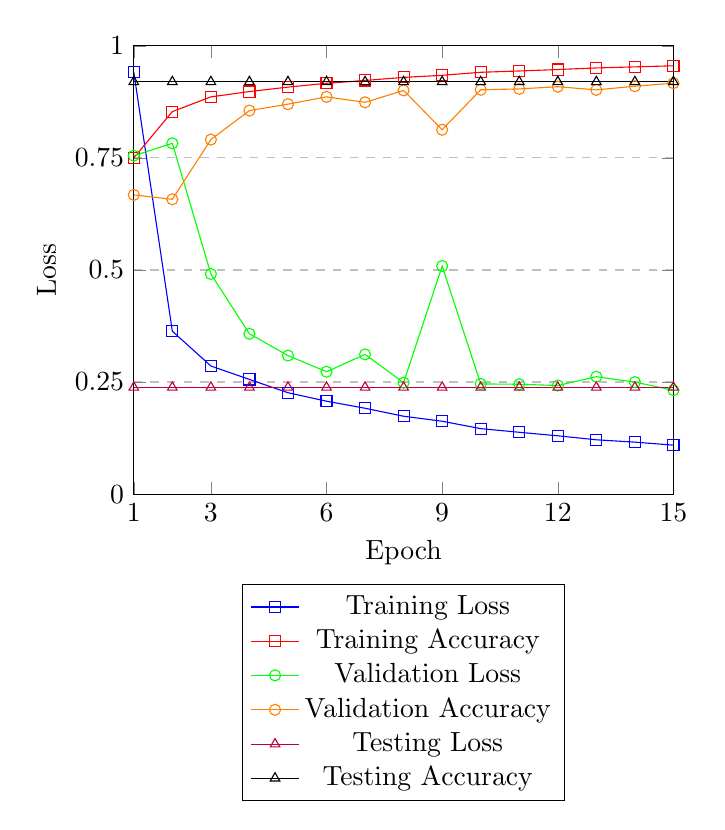
\begin{tikzpicture}
            \begin{axis}[
            xlabel={Epoch},
            ylabel={Loss},
            xmin=1, xmax=15,
            ymin=0, ymax=1,
            xtick={1, 3, 6, 9, 12, 15},
            ytick={0, .25, .50, .75, 1},
            legend style={at={(0.5,-0.2)},anchor=north},
            ymajorgrids=true,
            grid style=dashed,
            ]
                \addplot[
                color=blue,
                mark=square
                ]
                coordinates {
                (1, 0.9415369913395908)
                (2, 0.36347173816627926)
                (3, 0.2858551138391097)
                (4, 0.25580175934980315)
                (5, 0.22619957197457552)
                (6, 0.20731205224163002)
                (7, 0.19158202114825448)
                (8, 0.17376136417604154)
                (9, 0.1625804718480342)
                (10, 0.14612651362808216)
                (11, 0.1379509448694686)
                (12, 0.13010555795497364)
                (13, 0.12118976314862569)
                (14, 0.11594720014060537)
                (15, 0.10928217275068164)
                };
                \addplot[
                color=red,
                mark=square
                ]
                coordinates {
                (1, 0.7498944)
                (2, 0.8532715)
                (3, 0.8860656)
                (4, 0.8979578)
                (5, 0.90786415)
                (6, 0.9164315)
                (7, 0.9227066)
                (8, 0.9295607)
                (9, 0.9342024)
                (10, 0.94093925)
                (11, 0.94384027)
                (12, 0.9471116)
                (13, 0.9506346)
                (14, 0.9530575)
                (15, 0.9554094)
                };
                \addplot[
                color=green,
                mark=o
                ]
                coordinates {
                (1, 0.7549296505749226)
                (2, 0.7825332581996918)
                (3, 0.4910720940679312)
                (4, 0.357665928080678)
                (5, 0.3090804498642683)
                (6, 0.27299756929278374)
                (7, 0.31170774064958096)
                (8, 0.2485608123242855)
                (9, 0.508794916793704)
                (10, 0.24579987488687038)
                (11, 0.2450892459601164)
                (12, 0.24228437338024378)
                (13, 0.2619198402389884)
                (14, 0.24979994911700487)
                (15, 0.23182532005012035)
                };
                \addplot[
                color=orange,
                mark=o
                ]
                coordinates {
                (1, 0.66744876)
                (2, 0.6575944)
                (3, 0.79087156)
                (4, 0.8555428)
                (5, 0.86985517)
                (6, 0.88613117)
                (7, 0.8739339)
                (8, 0.9004858)
                (9, 0.81274575)
                (10, 0.901945)
                (11, 0.9038338)
                (12, 0.9087785)
                (13, 0.9017017)
                (14, 0.90983397)
                (15, 0.91657144)
                };
                \addplot[mark=triangle, color=purple]
                coordinates {
                (1, 0.23809038553127024)
                (2, 0.23809038553127024)
                (3, 0.23809038553127024)
                (4, 0.23809038553127024)
                (5, 0.23809038553127024)
                (6, 0.23809038553127024)
                (7, 0.23809038553127024)
                (8, 0.23809038553127024)
                (9, 0.23809038553127024)
                (10, 0.23809038553127024)
                (11, 0.23809038553127024)
                (12, 0.23809038553127024)
                (13, 0.23809038553127024)
                (14, 0.23809038553127024)
                (15, 0.23809038553127024)
                };
                \addplot[mark=triangle, color=black]
                coordinates {
                (1, 0.9196472)
                (2, 0.9196472)
                (3, 0.9196472)
                (4, 0.9196472)
                (5, 0.9196472)
                (6, 0.9196472)
                (7, 0.9196472)
                (8, 0.9196472)
                (9, 0.9196472)
                (10, 0.9196472)
                (11, 0.9196472)
                (12, 0.9196472)
                (13, 0.9196472)
                (14, 0.9196472)
                (15, 0.9196472)
                };
                \legend{Training Loss, Training Accuracy, Validation Loss, Validation Accuracy, Testing Loss, Testing Accuracy}
            \end{axis}
        \end{tikzpicture}
    \end{figure}

    \begin{figure}
        \caption{ACGAN Learning to Generate Clothing Images}
        \label{fig:results1}
        \centering
        \subfloat[\centering Epoch 1]{{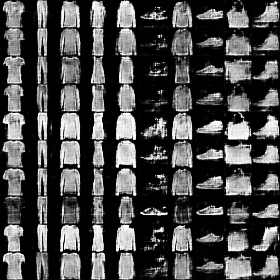
\includegraphics[width=2.5cm]{ACGAN_epoch001.png} }}
        \subfloat[\centering Epoch 25]{{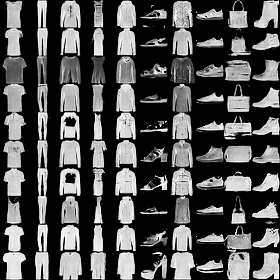
\includegraphics[width=2.5cm]{ACGAN_epoch025.png} }}
        \subfloat[\centering Epoch 50]{{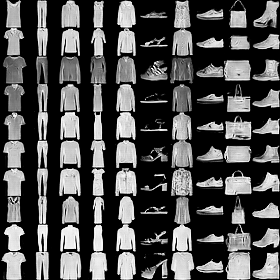
\includegraphics[width=2.5cm]{ACGAN_epoch050.png} }}
    \end{figure}

    \section{Conclusion}\label{sec:conclusion}
    \bibliographystyle{ieeetr}
    \bibliography{report}
\end{document}